%\title{LaTeX Portrait Poster Template}
%%%%%%%%%%%%%%%%%%%%%%%%%%%%%%%%%%%%%%%%%
% a0poster Portrait Poster
% LaTeX Template
% Version 1.0 (22/06/13)
%
% The a0poster class was created by:
% Gerlinde Kettl and Matthias Weiser (tex@kettl.de)
% 
% This template has been downloaded from:
% http://www.LaTeXTemplates.com
%
% License:
% CC BY-NC-SA 3.0 (http://creativecommons.org/licenses/by-nc-sa/3.0/)
%
%%%%%%%%%%%%%%%%%%%%%%%%%%%%%%%%%%%%%%%%%

%----------------------------------------------------------------------------------------
%	PACKAGES AND OTHER DOCUMENT CONFIGURATIONS
%----------------------------------------------------------------------------------------

\documentclass[a0,portrait]{a0poster}

\usepackage{multicol} % This is so we can have multiple columns of text side-by-side
\columnsep=100pt % This is the amount of white space between the columns in the poster
\columnseprule=3pt % This is the thickness of the black line between the columns in the poster

\usepackage[svgnames]{xcolor} % Specify colors by their 'svgnames', for a full list of all colors available see here: http://www.latextemplates.com/svgnames-colors

\usepackage{times} % Use the times font
%\usepackage{palatino} % Uncomment to use the Palatino font

\usepackage{graphicx} % Required for including images
\graphicspath{{figures/}} % Location of the graphics files
\usepackage{booktabs} % Top and bottom rules for table
\usepackage[font=small,labelfont=bf]{caption} % Required for specifying captions to tables and figures
\usepackage{amsfonts, amsmath, amsthm, amssymb} % For math fonts, symbols and environments
\usepackage{wrapfig} % Allows wrapping text around tables and figures

\begin{document}

%----------------------------------------------------------------------------------------
%	POSTER HEADER 
%----------------------------------------------------------------------------------------

% The header is divided into two boxes:
% The first is 75% wide and houses the title, subtitle, names, university/organization and contact information
% The second is 25% wide and houses a logo for your university/organization or a photo of you
% The widths of these boxes can be easily edited to accommodate your content as you see fit

\begin{minipage}[b]{0.75\linewidth}
\VeryHuge \color{NavyBlue} \textbf{Decision Trees in Machine Learning} \color{Black}\\ % Title
\Huge\textit{An Introduction}\\[2.4cm] % Subtitle
\huge \textbf{Nikita Masand}\\[0.5cm] 
Mentor: Prof. Pranav Nerurkar\\[0.5cm] % Author(s)
\huge Dept of Computer Engineering and IT, VJTI \\[0.4cm] % University/organization
\end{minipage}
%
\begin{minipage}[b]{0.25\linewidth}

\includegraphics[width=8 cm]{logo.jpeg}\ 
\end{minipage}

\vspace{1cm} % A bit of extra whitespace between the header and poster content

%----------------------------------------------------------------------------------------

\begin{multicols}{3} % This is how many columns your poster will be broken into, a portrait poster is generally split into 2 columns

%----------------------------------------------------------------------------------------
%	ABSTRACT
%----------------------------------------------------------------------------------------

\color{Navy} % Navy color for the abstract

\begin{abstract}
Decision tree methodology is a commonly used data mining method for establishing classification systems based on multiple covariates or for developing prediction algorithms for a target variable. This method classifies a population into branch-like segments that construct an inverted tree with a root node, internal nodes, and leaf nodes. The algorithm is non-parametric and can efficiently deal with large, complicated data sets without imposing a complicated parametric structure. This poster is an introduction to the widely used Decision Trees.
\end{abstract}
%----------------------------------------------------------------------------------------
%	INTRODUCTION
%----------------------------------------------------------------------------------------

\color{Black} % SaddleBrown color for the introduction
\section*{Introduction}
A decision tree is a tree where each node represents a feature(attribute), each link(branch) represents a decision(rule) and each leaf represents an outcome(categorical or continues value).
The whole idea is to create a tree for the entire data and process a single outcome at every leaf(or minimize the error in every leaf). The topmost decision node in a tree which corresponds to the best predictor called root node. Decision trees can handle both categorical and numerical data.Each feature of the data set becomes a root[parent] node, and the leaf[child] nodes represent the outcomes. The decision on which feature to split on is made based on resultant entropy reduction or information gain from the split.

%----------------------------------------------------------------------------------------
%	Splitting
%----------------------------------------------------------------------------------------

\color{Black} % DarkSlateGray color for the rest of the content

\section*{Splitting}
Only input variables related to the target variable are used to split parent nodes into purer child nodes of the target variable. Both discrete input variables and continuous input variables (which are collapsed into two or more categories) can be used. When building the model one must first identify the most important input variables, and then split records at the root node and at subsequent internal nodes into two or more categories or ‘bins’ based on the status of these variables. Characteristics that are related to the degree of ‘purity’ of the resultant child nodes (i. e. , the proportion with the target condition) are used to choose between different potential input variables; these characteristics include entropy, Gini index, classification error, information gain, gain ratio, and twoing criteria.
\begin{center}\vspace{1cm}
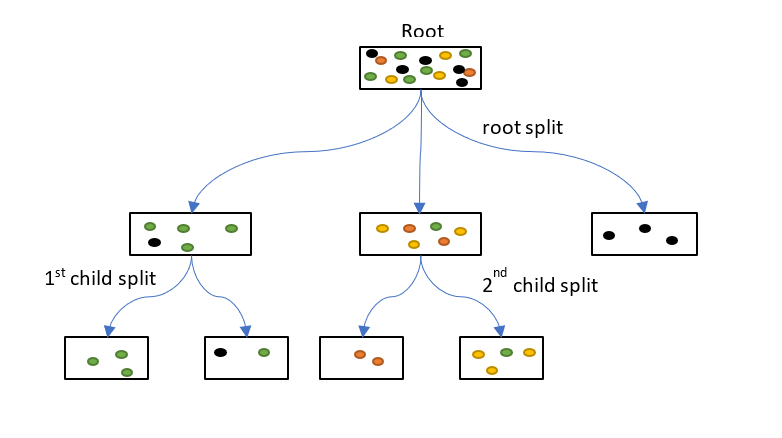
\includegraphics[width=0.8\linewidth]{decision-tree.png}
\captionof{figure}{\color{Green} Splitting in a tree}
\caption*{Source:https://www.displayr.com/how-is-splitting-decided-for-decision-trees/}
\end{center}%\vspace{1cm}
%----------------------------------------------------------------------------------------
%	Characteristics
%----------------------------------------------------------------------------------------
\section*{Characteristics}
\subsection*{Entropy}
\begin{itemize}
\item Entropy is the measure of impurity, disorder or uncertainty in a bunch of examples.
\item Entropy controls how a Decision Tree decides to split the data. It actually effects how a Decision Tree draws its boundaries.
\end{itemize}
\begin{center}\vspace{1cm}
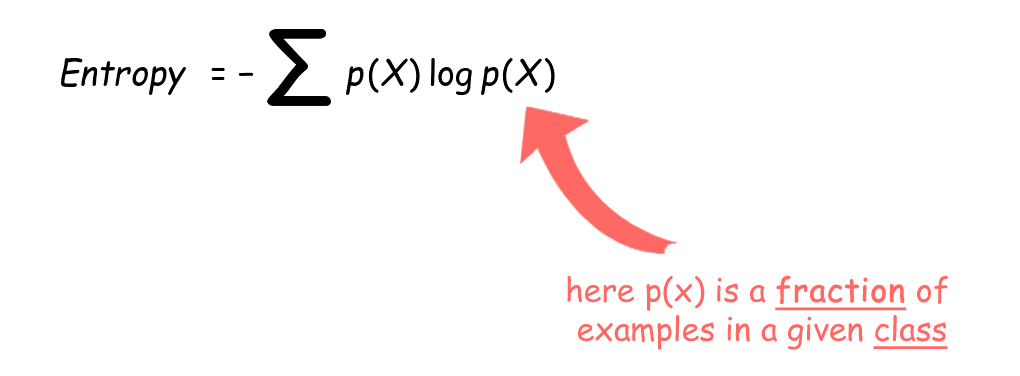
\includegraphics[width=1.0\linewidth]{entropy.png}
\captionof{figure}{\color{Green} Entropy}
\caption*{Source:https://www.saedsayad.com/decision_tree.htm}
\end{center}\vspace{1cm}

%------------------------------------------------

\subsection*{Information gain}
\begin{enumerate}
\item  Information gain (IG) measures how much “information” a feature gives us about the class.
\item Information gain is the main key that is used by Decision Tree Algorithms to construct a Decision Tree.
\item Decision Trees algorithm will always tries to maximize Information gain.
\item An attribute with highest Information gain will tested/split first.
\end{enumerate}
\begin{center}\vspace{1cm}
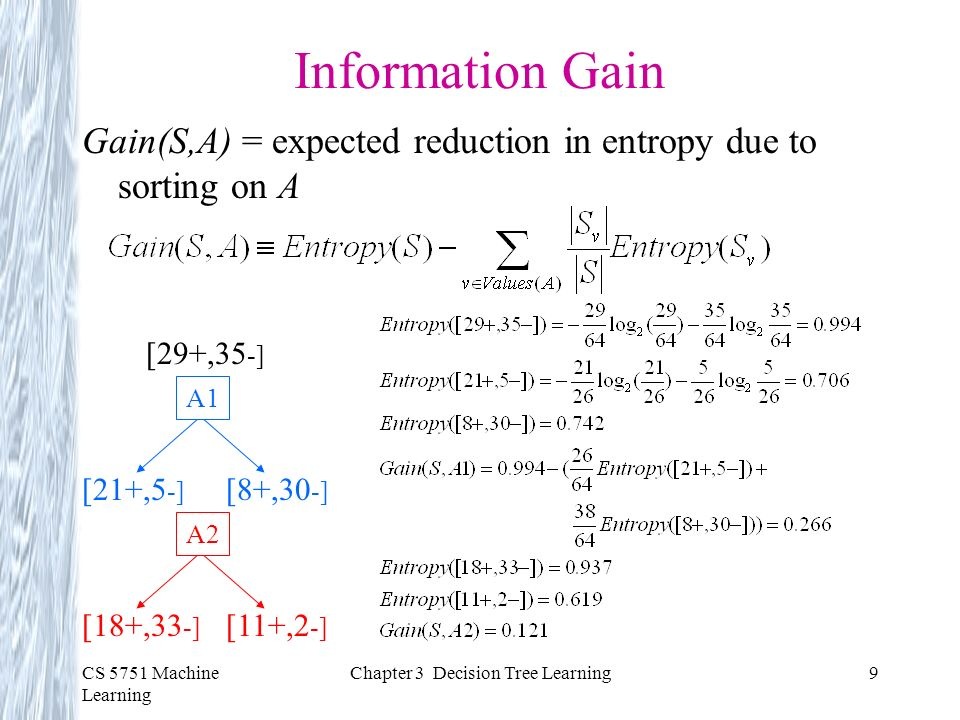
\includegraphics[width=0.8\linewidth]{gain.jpg}
\captionof{figure}{\color{Green} calculating information gain}
\caption*{Source:https://www.saedsayad.com/decisiontree.htm}
\end{center}\vspace{1cm}

\subsection*{Gini Index}
\begin{enumerate}
\item  Gini Index is a metric to measure how often a randomly chosen element would be incorrectly identified. It means an attribute with lower gini index should be preferred.
\item Gini index says, if we select two items from a population at random then they must be of same class and probability for this is 1 if population is pure.
\item It performs only Binary splits
Higher the value of Gini higher the homogeneity.
\item CART (Classification and Regression Tree) uses Gini method to create binary splits.
\end{enumerate}
\begin{center}\vspace{1cm}
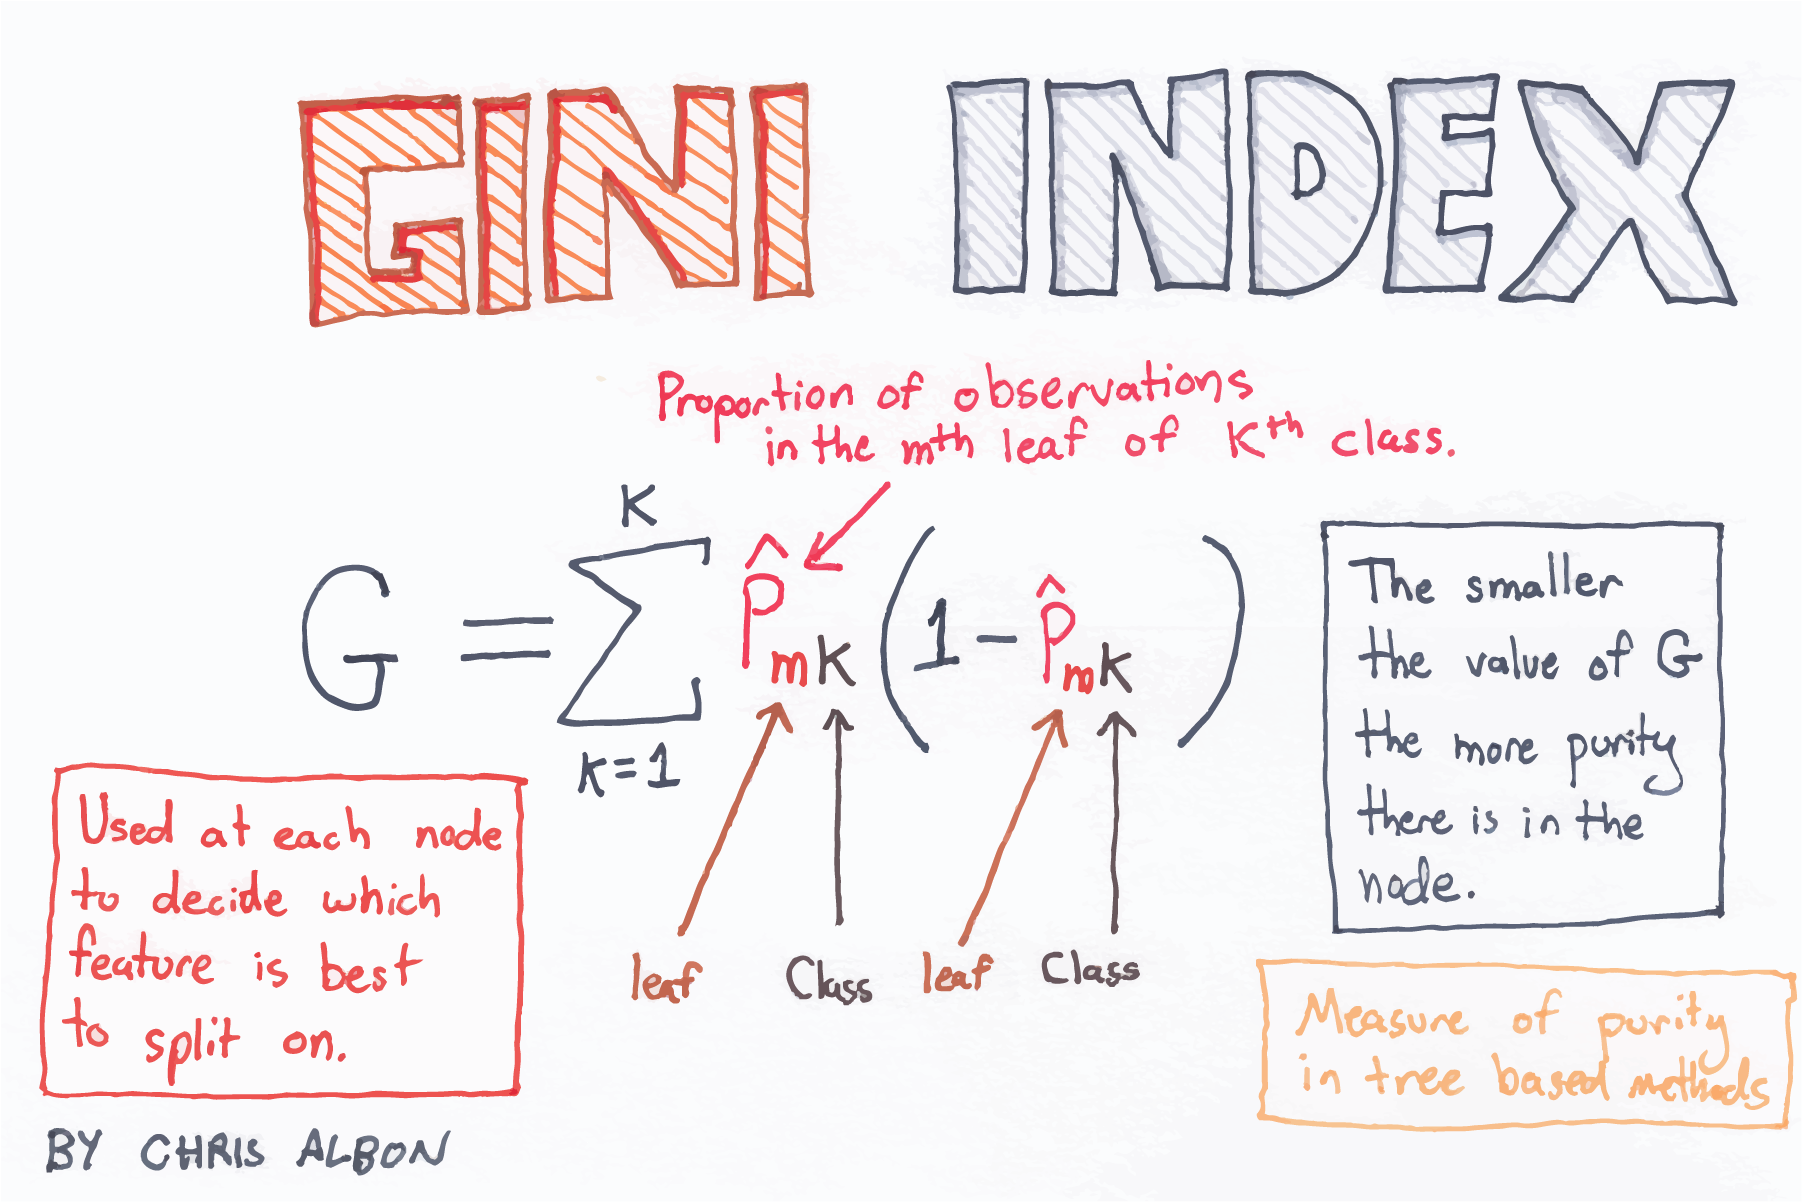
\includegraphics[width=0.8\linewidth]{Gini_Index_print.png}
\captionof{figure}{\color{Green}Gini Index}
\caption*{Source:https://t4tutorials.com/gini-index-data-mining/}
\end{center}\vspace{1cm}
\subsection*{CART-Classification And Regression Tree}
\begin{itemize}
\item The CART algorithm is structured as a sequence of questions, the answers to which determine what the next question, if any should be.
\item The result of these questions is a tree like structure where the ends are terminal nodes at which point there are no more questions.
\item The main elements of CART are:
\begin{enumerate}
    \item Rules for splitting data at a node based on the value of one variable
    \item Stopping rules for deciding when a branch is terminal and can be split no more
    \item Finally, a prediction for the target variable in each terminal node.
\end{enumerate}
\end{itemize}
\begin{center}\vspace{1cm}
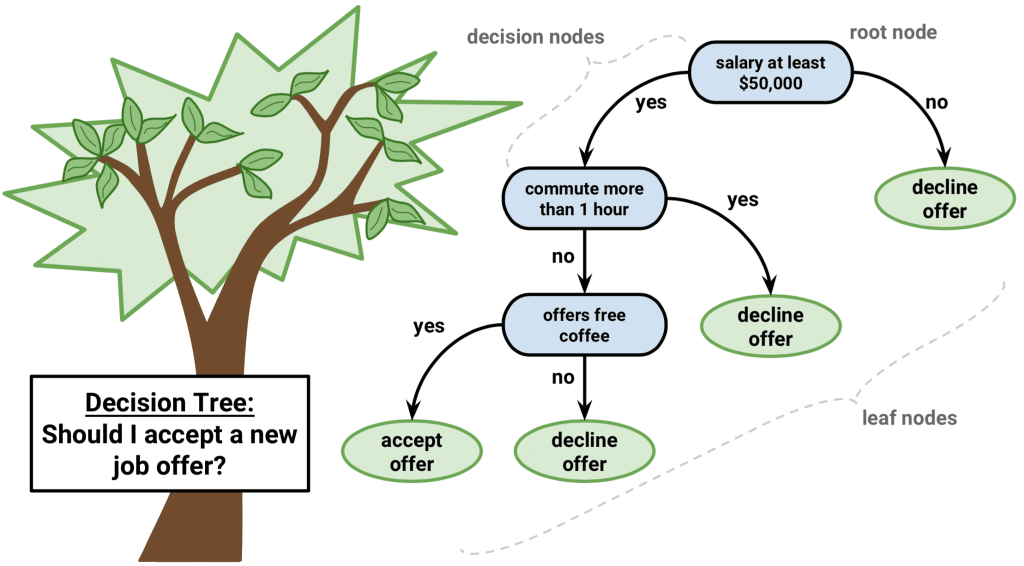
\includegraphics[width=0.8\linewidth]{exampletree.png}
\captionof{figure}{\color{Green}Decision tree CART}
\caption*{Source:https://machinelearningmastery.com/cart-for-machine-learning/}
\end{center}\vspace{1cm}

\subsection*{Pruning}
\begin{enumerate}
\item  As the name implies, pruning involves cutting back the tree. 
\item After a tree has been built it may be overfitted. The CART algorithm will repeatedly partition data into smaller and smaller subsets until those final subsets are homogeneous in terms of the outcome variable.
\end{enumerate}
\begin{center}\vspace{1cm}
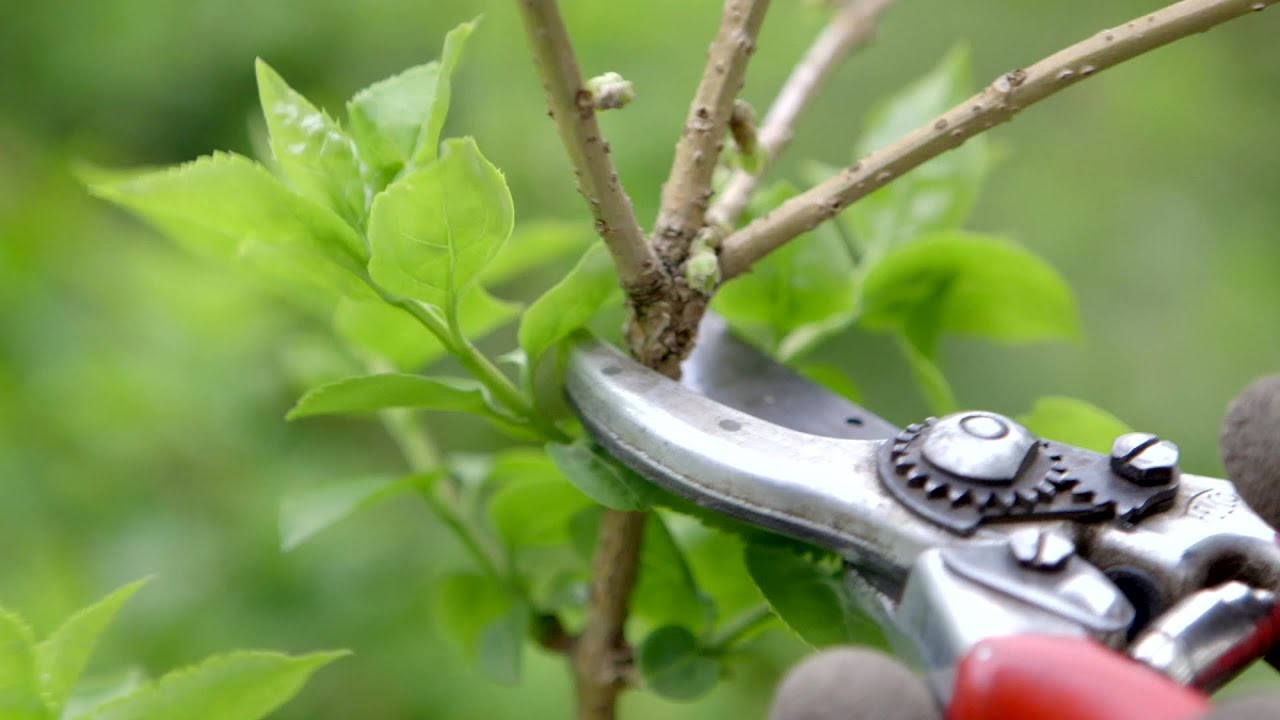
\includegraphics[width=1.0\linewidth]{prune.jpg}
\captionof{figure}{\color{Green}pruning}
\caption*{Source:https://www.finegardening.com/pruning-tips-and-techniques}
\end{center}

%----------------------------------------------------------------------------------------
%	Implementations
%----------------------------------------------------------------------------------------

\color{SaddleBrown} % SaddleBrown color for the implementations to make them stand out

\section*{Implementation}
Many data mining software packages provide implementations of one or more decision tree algorithms.
Examples include Salford Systems CART (which licensed the proprietary code of the original CART authors),[3] IBM SPSS Modeler, RapidMiner, SAS Enterprise Miner, Matlab, R (an open-source software environment for statistical computing, which includes several CART implementations such as rpart, party and randomForest packages), Weka (a free and open-source data-mining suite, contains many decision tree algorithms), Orange, KNIME, Microsoft SQL Server [1], and scikit-learn (a free and open-source machine learning library for the Python programming language).
\color{Black} % Set the color back to DarkSlateGray for the rest of the content

%----------------------------------------------------------------------------------------
%	FORTHCOMING RESEARCH
%----------------------------------------------------------------------------------------

\section*{Forthcoming Research}

In a decision tree, all paths from the root node to the leaf node proceed by way of conjunction, or AND. In a decision graph, it is possible to use disjunctions (ORs) to join two more paths together using minimum message length (MML). Decision graphs have been further extended to allow for previously unstated new attributes to be learnt dynamically and used at different places within the graph.[

 %----------------------------------------------------------------------------------------
%	REFERENCES
%----------------------------------------------------------------------------------------

\nocite{*} % Print all references regardless of whether they were cited in the poster or not
\bibliographystyle{plain} % Plain referencing style
\bibliography{sample} % Use the example bibliography file sample.bib

%----------------------------------------------------------------------------------------

\end{multicols}
\end{document}